\subsection{General}
The application is divided into two modes: free talk and interview. The former is for whom have their own speech material, while the later without material will be interviewed by other users. The audience are divided in three different characters: kind classmates \& colleagues, serious experts and indifferent people. Different character will give different feedback during the speech. The user could choose the number and composition of the audience.

\subsection{Audience}
\begin{itemize}
	\item Kind classmates \& colleagues: with causal wearing and friendly smile, they will listen with smile, nod and praise during the speech.
	\item Indifferent people: with strange wearing, they pay no attention to the speaker and will look around, speak to others and fall asleep during the speech.
	\item Serious experts: with formal suit and serious expression, they will listen without emotion, shake head and get angry during the speech.
\end{itemize}

\begin{figure}[H]
	\centering
	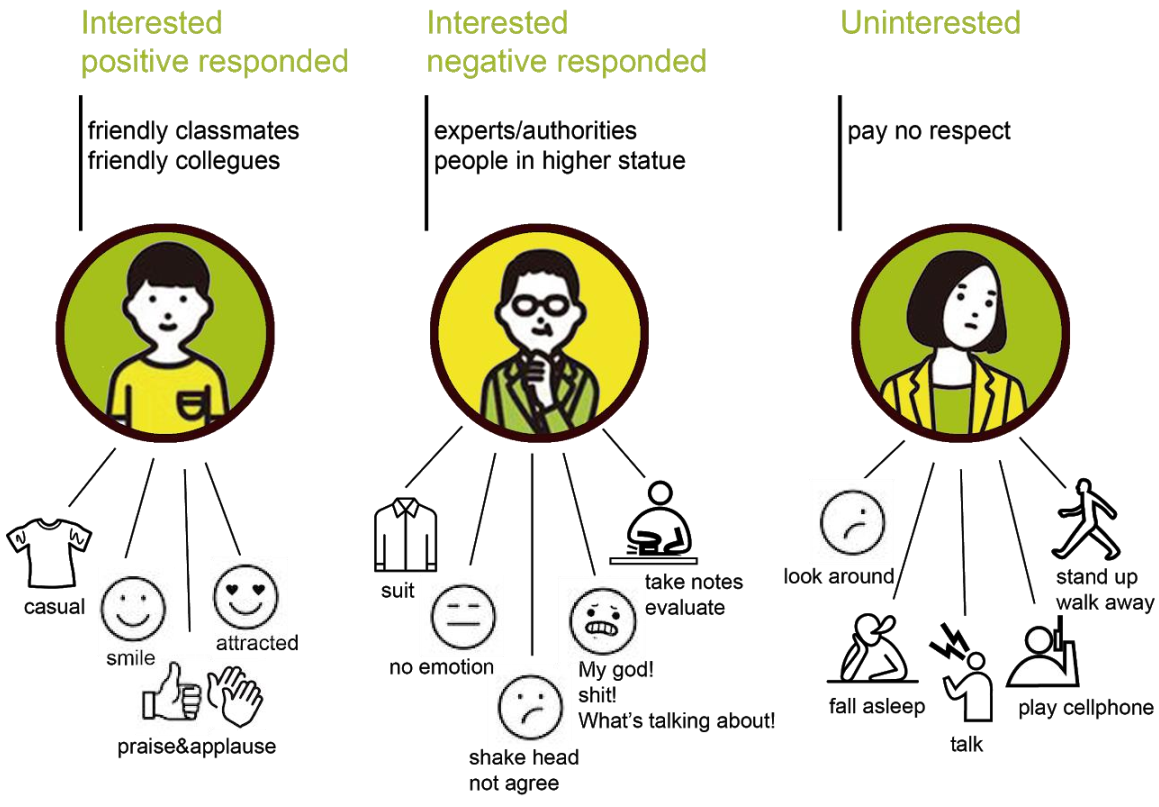
\includegraphics[scale=0.5]{Audience}
	\caption{Audience characteristics}
\end{figure}

\subsection{Audience number and composition}
\begin{itemize}
	\item Number: the number of audience will be changed by the light in the theater. More audience will come into view with bigger light.
	\item Composition: the users can choose different compositions of audience in different characters, which will help them to meet their own level.
\end{itemize}

\begin{figure}[H]
	\centering
	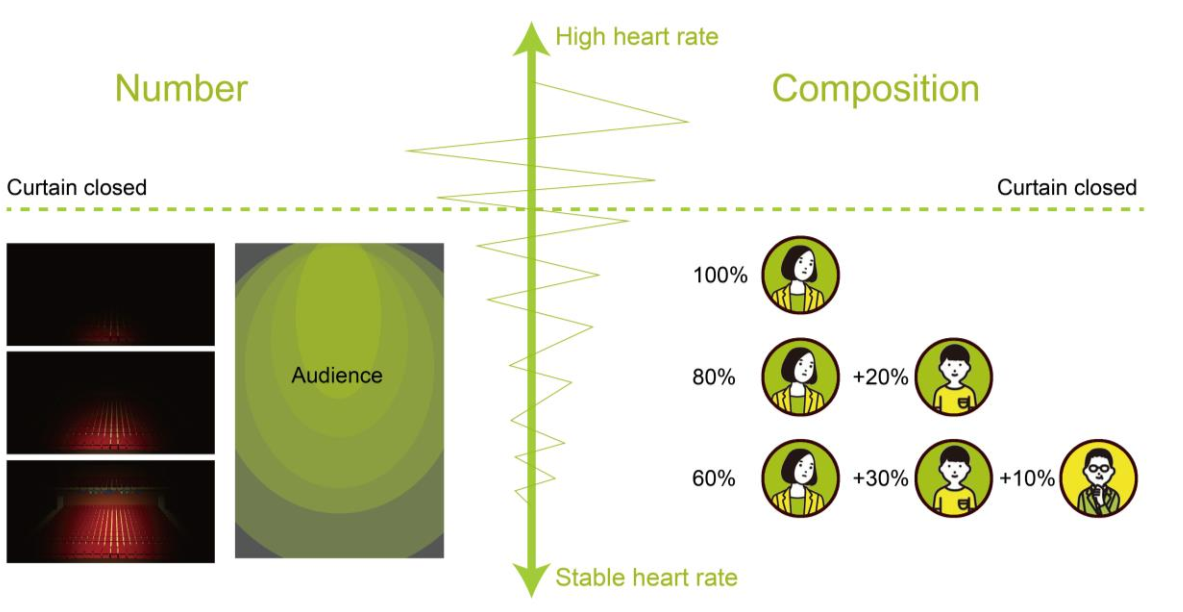
\includegraphics[scale=0.528]{Composition}
	\caption{Number and Composition}
\end{figure}

\subsection{Process}
\begin{figure}[H]
	\centering
	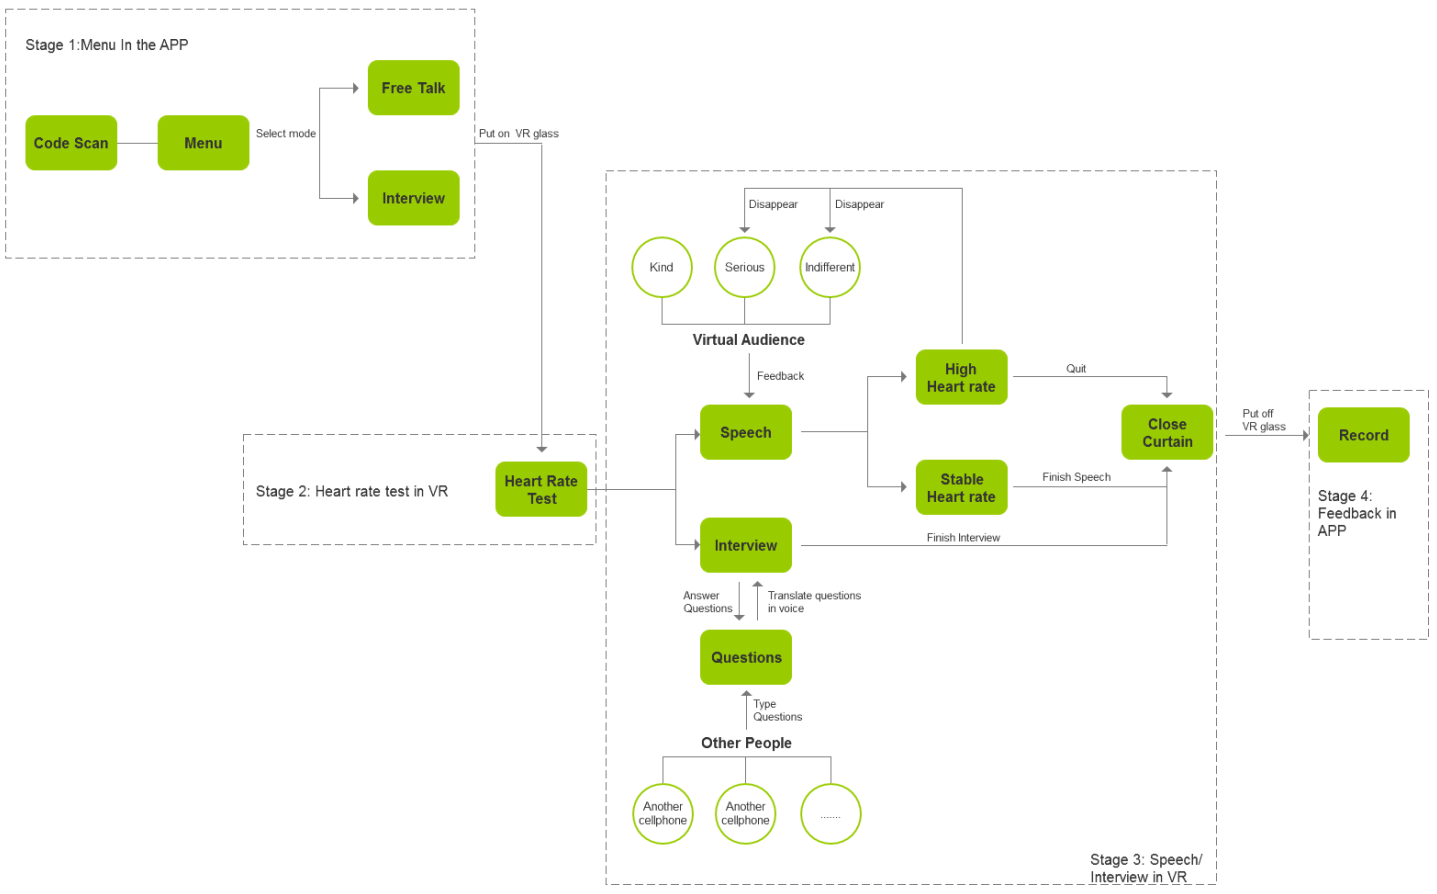
\includegraphics[scale=0.434]{Process}
	\caption{Flow of the application}
\end{figure}


\subsection{Interface}
\begin{figure}[H]
	\centering
	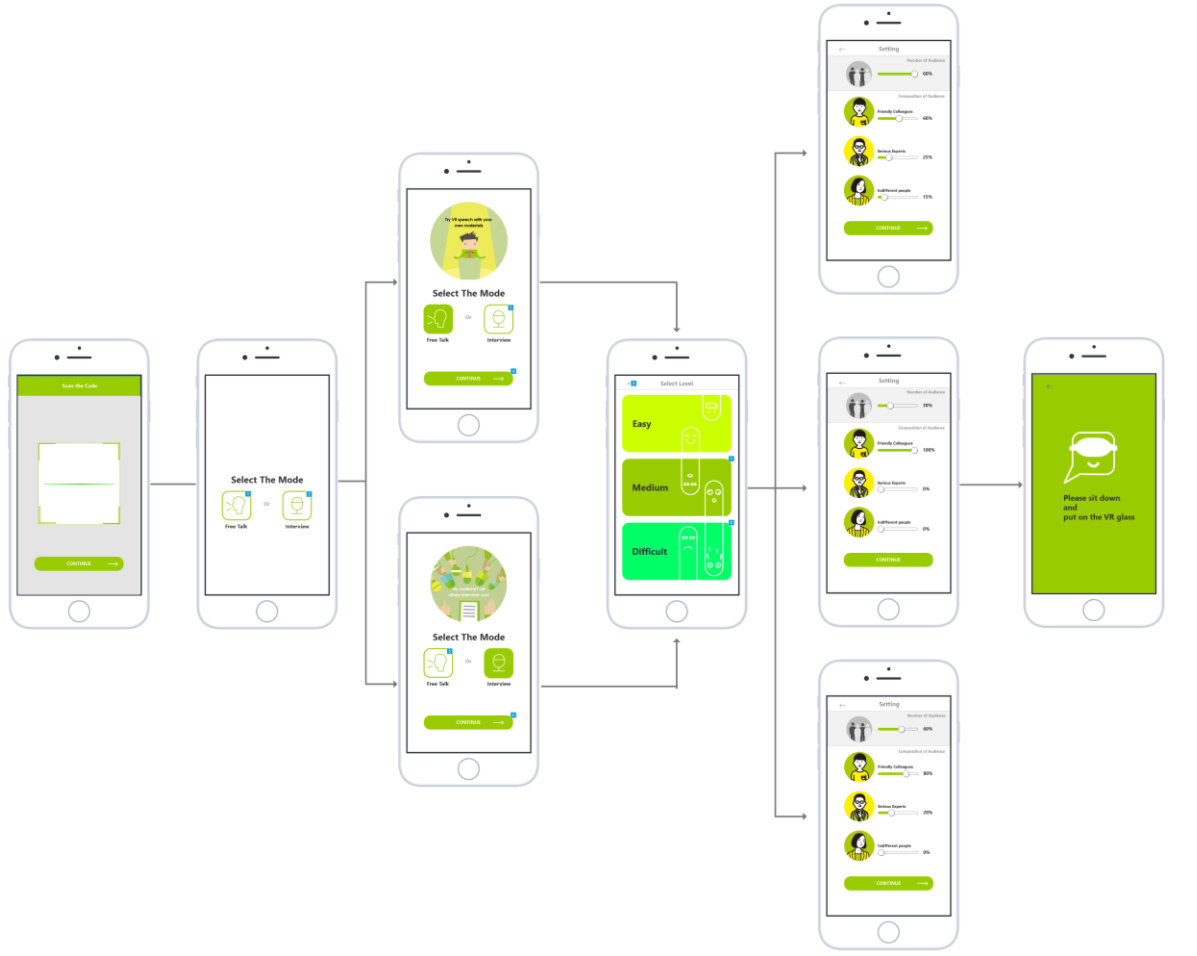
\includegraphics[scale=0.521]{Interface}
	\caption{Stage 1: App}
\end{figure}

\begin{figure}[H]
	\centering
	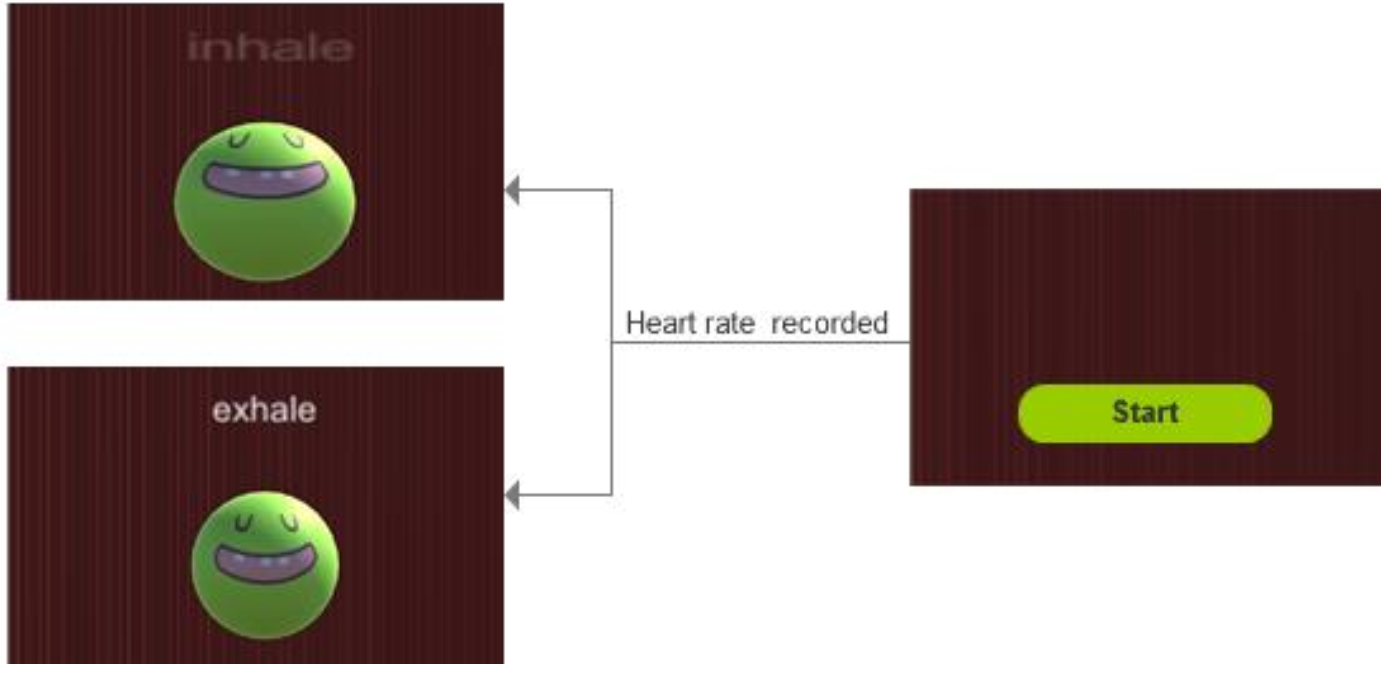
\includegraphics[scale=0.45]{Breathing}
	\caption{Stage 2: Heart rate test}
\end{figure}